\documentclass{beamer}

\usepackage{txfonts}
\usepackage{hyperref}
\usepackage{fancybox}
\usepackage{xfrac}
\usepackage{cancel}

\newcommand{\heart}{\ensuremath\heartsuit}

\usepackage{mathtools,amssymb}
\newcommand{\myarrow}{\scalebox{2}[2]{$\mathclap{\curvearrowleft}\mkern2.2mu
                                                 \mathclap{\curvearrowright}$}}

\DeclareMathOperator{\Bin}{\mathrm{Bin}}

\hypersetup{colorlinks=false,linkbordercolor=red,linkcolor=green,pdfborderstyle={/S/U/W 1}}

\addtobeamertemplate{navigation symbols}{}{ \hspace{1em}    \usebeamerfont{footline}%
    \insertframenumber / \inserttotalframenumber}

\geometry{papersize={15cm,13cm}}
\usepackage{lipsum}

\makeatletter
\newenvironment<>{contdproof}[1][\proofname]{%
    \par
    \def\insertproofname{#1\@addpunct{.}}%
    \usebeamertemplate{proof begin}#2}
  {\usebeamertemplate{proof end}}
\makeatother


\setbeamertemplate{theorems}[numbered]

\newtheorem*{nonumdefinition}{Definition}
\newtheorem*{nonumproblem}{Problem}
\newtheorem*{nonumproof}{Proof}
\newtheorem*{nonumtheorem}{Theorem}
\newtheorem*{nonumremark}{Remark}
\newtheorem*{answer}{Answer}
\newtheorem*{nonumremarks}{Remarks}
\newtheorem*{nonumexamples}{Examples}
\newtheorem*{nonumsolution}{Solution}
\newtheorem*{nonumexample}{Example}
\newtheorem*{nonumproposition}{Proposition}
\newtheorem{proposition}[theorem]{Proposition}

\usepackage{tikz}
\newcommand*\mycirc[1]{%
  \tikz[baseline=(C.base)]\node[draw,circle,inner sep=.7pt](C) {#1};\:
}

\newcommand\myheading[1]{%
  \par\bigskip
  {\color{blue}{\large #1}}\par\smallskip}

%\usetheme{Warsaw}
%\usetheme{Berkeley} %sample 1

\usetheme{Berlin} % sample 2
%\usetheme{AnnArbor} % sample 3

\let\otp\titlepage
\renewcommand{\titlepage}{\otp\addtocounter{framenumber}{-1}}

\title{Lecture 11 : The Basic Numerical Quantities Associated to a Continuous $X$}
\author{}
\date{}

\begin{document}
\begin{frame}[plain]
\titlepage
\end{frame}

\begin{frame}
In this lecture we will introduce four basic numerical quantities associated to a continuous random variable $X$. You will be asked to calculate these (and the $cdf$ of $X$) given $f(x)$ on the midterms and the final.

These quantities are
\begin{enumerate}
\item The $p$-th percentile $\eta(P)$.

\item The $\alpha$-th critical value $X_{\alpha}$.

\item The expected value $E(X)$ or $\mu$.

\item The variance $V(X)$ or $\sigma^{2}$.
\end{enumerate}
I will compute all these for $\cup(a,b)$ the linear distribution and $\cup(a,b)$.
\end{frame}

\begin{frame}
\myheading{Percentiles and Critical Values of Continuous Random Variables}

\myheading{Percentiles}

Let $P$ be a number between $0$ and $1$. The $100p$-th percentile, denoted $\eta(P)$, of a continuous random variable $X$ is the unique number satisfying
\begin{equation*}
P(X\leq \eta(P))=P\tag{$\sharp$}
\end{equation*}
or
\begin{equation*}
F(\eta(P))=P\tag{$\sharp\sharp$}
\end{equation*}
So if you know $F$ you can find $\eta(P)$. Roughly
$$
\eta (P)=F^{-1}(P)
$$
\end{frame}

\begin{frame}
The geometric interpretation of $\eta(P)$ is very important

\medskip
\centerline{
\includegraphics{figure/fig1.eps}}
\smallskip

\myheading{The geometric interpretation of $(\sharp)$}

$\eta(P)$ is the number such that the vertical line $x=\eta(P)$ cuts off area $P$ to the left under the graph of $f(x)$.

(this is the picture above)
\end{frame}

\begin{frame}
\myheading{Special Case\quad The median $\widetilde{\mu}$}

The median $\widetilde{\mu}$ is the unique number so that
\begin{align*}
P(X\leq \widetilde{\mu}) &= \frac{1}{2}\\[3pt]
\text{or}\qquad F(\widetilde{\mu}) &= \frac{1}{2}
\end{align*}
so the median is the 50-th percentile.

\myheading{The picture}

\centerline{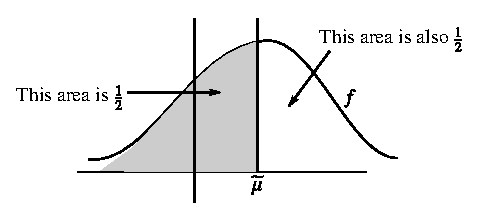
\includegraphics{figure/fig2.eps}}
\smallskip

Since the total area is 1, the area to the right of the vertical line $x=\widetilde{\mu}$ also $\dfrac{1}{2}$. So $x=\widetilde{\mu}$ bisects the area.
\end{frame}

\begin{frame}
\myheading{Critical Values}

Roughly speaking if you switch left to right in the definition of percentile you get the definition of the critical value. Critical values play a key role in the formulas for {\it confidence intervals} (later).

\begin{nonumdefinition}
Let $\alpha$ be a real number between $0$ and $1$. Then the $\alpha$-th critical value, denoted $x_{\alpha}$, is the unique number satisfying
\begin{equation*}
P(X\geq x_{\alpha})=\alpha\tag{b}
\end{equation*}
\end{nonumdefinition}
\end{frame}

\begin{frame}
Let's rewrite (b) in terms of $F$. We have
\begin{align*}
P(X\geq x_{\alpha}) &= 1-P(X\leq x_{\alpha})\\[3pt]
                  &= 1-F(x_{\alpha})
\end{align*}
So (b) becomes
\begin{align*}
& 1-F(x_{\alpha})=\alpha\\
& F(x_{\alpha})=1-\alpha\\
& x_{\alpha} = F^{-1}(1-\alpha)\tag{bb}
\end{align*}
What about the geometric interpretation?
\end{frame}

\begin{frame}
\myheading{The geometric interpretation}

\smallskip
\centerline{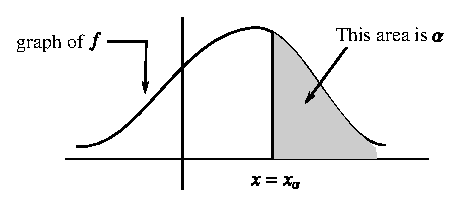
\includegraphics{figure/fig3.eps}}
\smallskip

$x_{\alpha}$ is the number so that the vertical line $x=x_{\alpha}$ cuts off area $\alpha$ to the {\it right} under the graph of $f(x)$.

\myheading{Relation between critical values and percentiles}

$x=x_{\alpha}$ cuts off area $1-\alpha$ to the {\it left} since the total area is 1. But $n(1-\alpha)$ is the number such that $x=\eta(1-\alpha)$ cuts off area $1-\alpha$ to the left.

So
$$
\underline{x_{\alpha}=\eta(1-\alpha)}
$$
\end{frame}

\begin{frame}
\myheading{Computation of Examples}

\begin{example}[$X\sim \bigcup(a,b)$]
Lets compute the $\eta(p)$-th percentile for $X\sim \bigcup (a,b)$

\medskip
\centerline{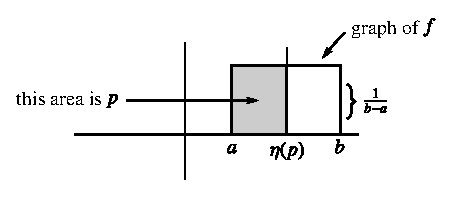
\includegraphics{figure/fig4.eps}}
\smallskip

So the point $\eta(p)$ between $a$ and $b$ must have the property that the area of the shaded box is $p$. But the base of the box is $\eta(p)-a$ and the height is $\dfrac{1}{h-a}$ so
\begin{gather*}
\text{Area} = bh = (\eta(p)-a)\left(\dfrac{1}{b-a}\right)\quad\text{so}\\
(n(p)-a)\left(\frac{1}{b-a}\right)=p\quad\text{or}\\
\eta(p)=a+p(b-a)=(1-p)a+pb\tag{*}
\end{gather*}
\end{example}
\end{frame}

\begin{frame}
\setcounter{theorem}{0}
\begin{example}[Cont.]
How about the median $\widetilde{\mu}$.

So we want $\eta(\frac{1}{2})$. By (*) we have
$$
\widetilde{\mu}=\eta\left(\dfrac{1}{2}\right)-a+\frac{b-a}{2}=\dfrac{a+b}{2}
$$
\end{example}

\begin{nonumremark}
$\dfrac{a+b}{2}$ is the midpoint of the interval $[a,b]$.

\medskip
\centerline{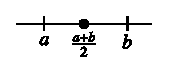
\includegraphics{figure/fig5.eps}}
\end{nonumremark}
\end{frame}

\begin{frame}
\myheading{Critical Values for $\bigcup(a,b)$}
\begin{align*}
x_{\alpha} &= \eta(1-\alpha)=a+(1-\alpha)(b-\alpha)\\[3pt]
         &= a+b-a-\alpha b +\alpha a\\[3pt]
\text{So}\quad x_{\alpha} &= \alpha a + (1-\alpha)b.
\end{align*}

\begin{example}[The linear distribution]
Recall the linear distribution has density
$$
f(x)=
\begin{array}{cl}
0, & x<0\\
2x, & 0\leq x\leq 1\\
0, & x>1
\end{array}
$$

\centerline{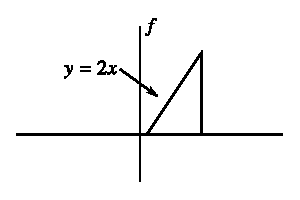
\includegraphics{figure/fig6.eps}}
\end{example}
\end{frame}

\begin{frame}
\myheading{The $100p$-th percentile}

\centerline{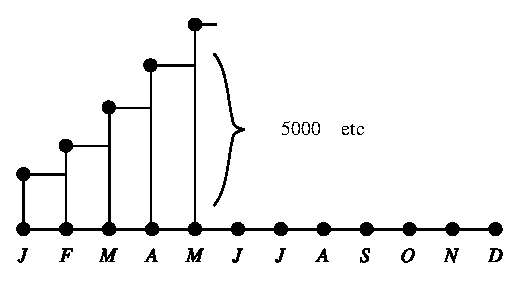
\includegraphics{figure/fig7.eps}}

We want the area of the triangle to be $p$. But the box is $\eta(p)$ and the height is $Z\eta(p)$ so 
\begin{align*}
A=\frac{1}{2}bh &= \frac{1}{2}\eta(p)(2n(p))\\
                &= \eta(p)^{2}
\end{align*}
We have to solve
\begin{align*}
\eta(p)^{2} &= p\\
\text{So}\quad \eta(p) &= \sqrt{p}
\end{align*}
\end{frame}

\begin{frame}
In particular
$$
\widetilde{\mu} =\eta\left(\frac{1}{2}\right)=\sqrt{\frac{1}{2}}=\frac{\sqrt{2}}{2}
$$
This will be important later.
\end{frame}

\begin{frame}
\myheading{Expected Value}

\begin{nonumdefinition}
The expected value or mean $E(X)$ or $\mu$ of a continuous random variable is defined by 
$$
E(X)=\int\limits^{\infty}_{-\infty}xf(x)dx
$$
We will compute some examples.
\end{nonumdefinition}

\setcounter{theorem}{0}
\begin{example}[$X\sim \bigcup (a,b)$]
\begin{align*}
E(X) &= \int\limits^{\infty}_{-\infty}f(x)dx=\int\limits^{b}_{a}\frac{1}{b-a}x \ dx\\
&= \frac{1}{b-a}\left.\left(\frac{x^{2}}{2}\right)\right|^{x-b}_{x=a}=\frac{1}{2}\frac{(b^{2}-a^{2})}{b-a}=\frac{b+a}{2}
\end{align*}
\end{example}
\end{frame}

\begin{frame}
\setcounter{theorem}{0}
\begin{example}[Cont.]
Now we showed on page 9 that if $X\sim \bigcup (a,b)$ then the median $\widetilde{\mu}$ was given by $\widetilde{\mu}=\dfrac{a+b}{2}$.

Hence in this {\it the mean is equal to the median}
$$
\mu=\widetilde{\mu}=\dfrac{a+b}{2}
$$
\end{example}

\begin{itemize}
\item[\dbend] This is not always the case as we will see shortly.
\end{itemize}
\end{frame}

\begin{frame}
The ``reason'' $\mu=\widetilde{\mu}$ is that $f(x)$ has a point of symmetry i.e. a point $x_{0}$ so that $f(x_{0}fy)=f(x_{0}-y)$

\medskip
\centerline{
\includegraphics{figure/fig8.eps}}
\smallskip

This means that the graph is symmetrical about the vertical line (mirror) $x=x_{0}$.

\begin{nonumproposition}[Useful fact]
If $x_{0}$ is a point of symmetry for $f(x)$ then
$$
\mu=\widetilde{\mu}=x_{0}
$$
\end{nonumproposition}
\end{frame}

\begin{frame}
\begin{nonumproposition}[Cont.]
Now if $X\sim \bigcup (a,b)$ then $x_{0}=\dfrac{a+b}{2}$ is a point of symmetry for $f(x)$

\medskip
\centerline{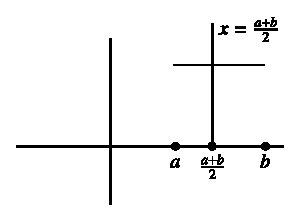
\includegraphics{figure/fig9.eps}}
\end{nonumproposition}

For a change we will prove the proposition

\begin{nonumproof}
$\widetilde{\mu}=x_{0}$ is immediate because by symmetry there is equal area to the left and right of $x_{0}$.
\end{nonumproof}
\end{frame}

\begin{frame}
\begin{nonumproof}[Cont.]
\centerline{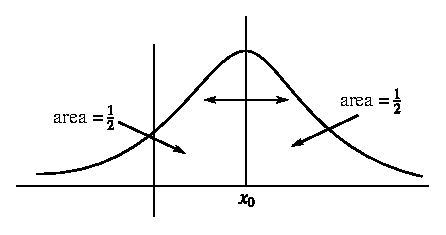
\includegraphics{figure/fig10.eps}}
\smallskip

Since the total area is 1, the area to the left of $x_{0}$ is $\dfrac{1}{2}$. 

Hence $\widetilde{\mu}=x_{0}$.

It is harder to prove
$$
E(X)=\int\limits^{\infty}_{-\infty}xf(x)=x_{0}
$$
Trick : Since $x_{0}$ is a constant and $\int^{\infty}_{-\infty}f(x)dx=1$ we have
$$
\int\limits^{\infty}_{-\infty}x_{0} f(x)dx=x_{0}
$$
\end{nonumproof}
\end{frame}

\begin{frame}
\begin{nonumproof}[Cont.]
Thus to show
$$
\int\limits^{\infty}_{-\infty}xf(x)dx=x_{0}
$$
It suffices to show
$$
\int\limits^{\infty}_{-\infty}xf(x)dx=\int\limits^{\infty}_{-\infty}x_{0}f(x)dx
$$
or
$$
\int\limits^{\infty}_{-\infty}(x-x_{0})f(x)dx=0
$$
But if we put
$$
g(x)=(x-x_{0})f(x)\quad\text{then}
$$
$g(x)$ is antisymmetric or ``odd'' about $x_{0}$
$$
g(x_{0}+y)=-g(x_{0}+g)
$$
\end{nonumproof}
\end{frame}

\begin{frame}
\begin{proof}[Proof (Cont.)]
This is because $x-x_{0}$ is

\medskip
\centerline{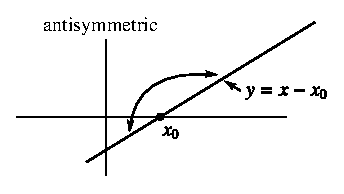
\includegraphics{figure/fig11.eps}}
\smallskip

But antisymmetric symmetric = antisymmetric (or odd-even = odd).

Finally the integral of on antisymmetric (or ``odd'') function from $-\infty$ to $\infty$ is zero.

\medskip
\centerline{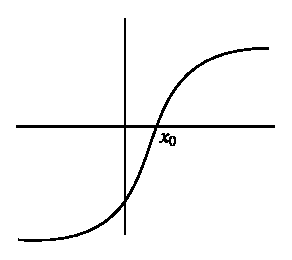
\includegraphics{figure/fig12.eps}}
\smallskip

The integral to the left of $x_{0}$ cancels the area to the right.
\end{proof}
\end{frame}

\begin{frame}
This fact can save a lot of painful computation of expected values.

\begin{example}[The linear distribution]

\centerline{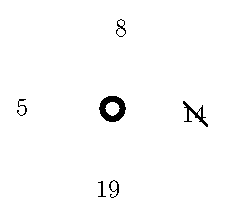
\includegraphics{figure/fig13.eps}}

We have seen $\widetilde{\mu}=\dfrac{\sqrt{2}}{2}$, page 12, $f(x)$ is certainly not symmetric so it is possible $\mu=\widetilde{\mu}$ and we will see that it is the case.
\end{example}
\end{frame}

\begin{frame}
\begin{align*}
E(X) &= \int\limits^{\infty}_{-\infty}xf(x)dx\\
     &= \int\limits^{1}_{0}x(2x)dx\\
     &= 2\int\limits^{1}_{0}x^{2}\ dx\\
     &= 2\left(\dfrac{1}{3}\right)=\dfrac{2}{3}
\end{align*}
Handy fact \ $\int^{1}_{0} x^{n}=\dfrac{1}{n}$.

So \ $\mu=\dfrac{2}{3}$ and $\widetilde{\mu}=\dfrac{2}{\sqrt{2}}$.

They aren't equal, which one is bigger?
\end{frame}

\begin{frame}
\myheading{Variance}

The variance $V(X)$ or $\sigma^{2}$ of a continuous random variable is defined by
$$
V(X)=\int\limits^{\infty}_{-\infty}(x-\mu)^{2}f(x)dx
$$

\begin{nonumremark}
Once we learn about change of continuous random variable we will see this is

\medskip
\centerline{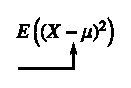
\includegraphics{figure/fig14.eps}}
\smallskip

new random variable obtains from $X$ using $h(x)=(x-\mu)^{2}$.
\end{nonumremark}
\end{frame}

\begin{frame}
Once again there is a shortcut formula for $V(X)$.

\begin{nonumproposition}[Shortcut Formula]
\begin{align*}
V(X) &= E(X^{2})-(E(X))^{2}\\
     &= E(X^{2})-\mu^{2}
\end{align*}
\end{nonumproposition}

\myheading{This is the formula to use}

\setcounter{theorem}{0}
\begin{example}[$X\sim \bigcup(a,b)$]
We know $\mu=\dfrac{a+b}{2}$. We have to compute $E(X^{2})$
\end{example}
\end{frame}

\begin{frame}
\setcounter{theorem}{0}
\begin{example}[Cont.]
\begin{align*}
E(X^{2}) &= \int\limits^{\infty}_{-\infty}x^{2}f(x)dx\\
&= \int\limits^{b}_{a}x^{2}{\displaystyle{\mathop{\perp}\limits_{b-a}}} dx\\
&= \frac{1}{b-a}\left.\left(\dfrac{x^{3}}{3}\right)\right|^{x=b}_{x=a}\\
&= \frac{1}{3}\frac{b^{3}-a^{3}}{b-a}=\frac{1}{3}(b^{2}+ab+a^{2})
\end{align*}
\centerline{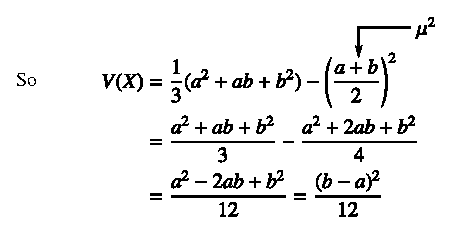
\includegraphics{figure/fig15.eps}}
\end{example}
\end{frame}

\begin{frame}
\begin{example}[The linear distribution]
We have seen (pg. 21)
$$
\mu=\dfrac{2}{3}
$$
We need $E(X^{2})$
\begin{align*}
E(X^{2}) &= \int\limits^{\infty}_{-\infty}X^{2}f(x)dx\\
        &= \int\limits^{1}_{0}x^{2}(2x)dx\\
        &= 2\int\limits^{1}_{0}x^{3}dx=2\left(\dfrac{1}{4}\right)=\frac{1}{2}\\
\text{SO}\qquad V(X) &= \frac{1}{2}-\left(\frac{2}{3}\right)^{2}=\frac{1}{2}-\frac{4}{9}\\
     &= \frac{9}{18}-\frac{8}{18}=\frac{1}{18}
\end{align*}
\end{example}
\end{frame}

\end{document}


